\subsection{Movimiento Horizontal}

\subsubsection{Parámetros del Sistema}

El sistema de movimiento horizontal utiliza una transmisión por correa dentada GT2 con las siguientes especificaciones:

\begin{itemize}
    \item \textbf{Carga total:} $m = 3.5$ kg
    \item \textbf{Longitud de la correa:} $L = 2.84$ m (eq. \ref{eq:longitud_correa})
    \item \textbf{Diámetro de poleas:} $D_p = 12$ mm y 20 dientes
    \item \textbf{Radio de poleas:} $r = 6$ mm = $0.006$ m
    \item \textbf{Ancho de la correa:} $b = 10$ mm
    \item \textbf{Paso de la correa GT2:} $p = 2$ mm
\end{itemize}

\subsubsection{Desplazamiento Lineal por Revolución}

El desplazamiento lineal del carro por cada revolución completa del motor es:

\begin{equation}
    d_{rev} = N_d \cdot p = 20 \cdot 2 = 40 \text{ mm/rev}
\end{equation}

\subsubsection{Cálculo de Fuerzas Actuantes}

\paragraph{Fuerza de Aceleración}

Considerando una aceleración deseada de $a = 0.5$ m/s$^2$ (valor típico para aplicaciones de posicionamiento preciso):

\begin{equation}
    F_a = m \cdot a = 3.5 \cdot 0.5 = 1.75 \text{ N}
\end{equation}

\paragraph{Fuerza de Fricción}

La fuerza de fricción se calcula con un coeficiente de fricción dinámico típico para carros con rodamientos lineales ($\mu = 0.02$):

\begin{equation}
    F_f = \mu \cdot m \cdot g = 0.02 \cdot 3.5 \cdot 9.81 = 0.69 \text{ N}
\end{equation}

\paragraph{Fuerza Total Requerida}

La fuerza total que debe ejercer el motor es la suma de la fuerza de aceleración y la fuerza de fricción:

\begin{equation}
    F_{total} = F_a + F_f = 1.75 + 0.69 = 2.44 \text{ N}
\end{equation}

\subsubsection{Torque Requerido en el Motor}

El torque necesario en el eje del motor se calcula multiplicando la fuerza total por el radio de la polea:

\begin{equation}
    T_{req} = F_{total} \cdot r = 2.44 \cdot 0.006 = 0.01464 \text{ N·m} = 14.64 \text{ mN·m}
\end{equation}

Expresado en kg·cm (unidad común en especificaciones de motores):

\begin{equation}
    T_{req} = \frac{0.01464}{0.0981} = 0.149 \text{ kg·cm} \approx 0.15 \text{ kg·cm}
\end{equation}

Para garantizar un funcionamiento confiable del sistema, se aplica un factor de seguridad de 2.5 a 3:

\begin{equation}
    T_{motor} = T_{req} \cdot FS = 0.15 \cdot 2.5 = 0.375 \text{ kg·cm}
\end{equation}

\subsubsection{Selección del Motor}

Considerando el torque calculado con factor de seguridad, se selecciona el motor paso a paso Nema 17 medium que posee  0.45Nm a 24V y 1.8A. 

\subsubsection{Resolución de Posicionamiento}

Con microstepping de 8 pasos (configuración típica con driver TB6600):

\begin{equation}
    \text{Pasos totales/rev} = 200 \cdot 8 = 1600 \text{ pasos/rev}
\end{equation}

\begin{equation}
    \text{Resolución} = \frac{d_{rev}}{\text{Pasos totales/rev}} = \frac{40}{1600} = 0.025 \text{ mm/paso}
\end{equation}

\subsubsection{Velocidad Máxima del Sistema}

Considerando una velocidad angular máxima del motor de 300 RPM (valor conservador para NEMA 17):

\begin{equation}
    v_{max} = \frac{300 \cdot 40}{60000} = 0.2 \text{ m/s} = 200 \text{ mm/s}
\end{equation}
Como se puede observar en la figura \ref{fig:Curva_din_nema17medium} para la velocidad máxima se cumple con el torque necesario.
\begin{figure}[H]
    \centering
    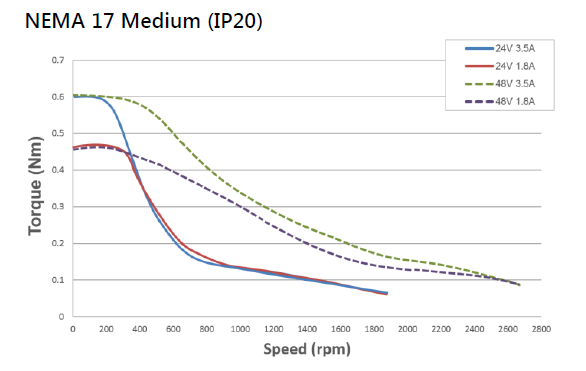
\includegraphics[width=0.65\textwidth]{img/nema17_medium.png}
    \caption{\textit{Curva dinámica torque-velocidad del motor paso a paso NEMA 17 para el prototipo.}}
    \label{fig:Curva_din_nema17medium}
\end{figure}
Como se cuentan con motores paso a paso que poseen 0.22Nm de torque se opta utilizar una configuración de dos motores, por lo que cada polea está acoplada a un motor. De esta manera se obtiene el torque final necesario a aplicar como la suma de los torques de ambos motores.